\documentclass[twoside]{book}

% Packages required by doxygen
\usepackage{fixltx2e}
\usepackage{calc}
\usepackage{doxygen}
\usepackage[export]{adjustbox} % also loads graphicx
\usepackage{graphicx}
\usepackage[utf8]{inputenc}
\usepackage{makeidx}
\usepackage{multicol}
\usepackage{multirow}
\PassOptionsToPackage{warn}{textcomp}
\usepackage{textcomp}
\usepackage[nointegrals]{wasysym}
\usepackage[table]{xcolor}

% Font selection
\usepackage[T1]{fontenc}
\usepackage[scaled=.90]{helvet}
\usepackage{courier}
\usepackage{amssymb}
\usepackage{sectsty}
\renewcommand{\familydefault}{\sfdefault}
\allsectionsfont{%
  \fontseries{bc}\selectfont%
  \color{darkgray}%
}
\renewcommand{\DoxyLabelFont}{%
  \fontseries{bc}\selectfont%
  \color{darkgray}%
}
\newcommand{\+}{\discretionary{\mbox{\scriptsize$\hookleftarrow$}}{}{}}

% Page & text layout
\usepackage{geometry}
\geometry{%
  a4paper,%
  top=2.5cm,%
  bottom=2.5cm,%
  left=2.5cm,%
  right=2.5cm%
}
\tolerance=750
\hfuzz=15pt
\hbadness=750
\setlength{\emergencystretch}{15pt}
\setlength{\parindent}{0cm}
\setlength{\parskip}{3ex plus 2ex minus 2ex}
\makeatletter
\renewcommand{\paragraph}{%
  \@startsection{paragraph}{4}{0ex}{-1.0ex}{1.0ex}{%
    \normalfont\normalsize\bfseries\SS@parafont%
  }%
}
\renewcommand{\subparagraph}{%
  \@startsection{subparagraph}{5}{0ex}{-1.0ex}{1.0ex}{%
    \normalfont\normalsize\bfseries\SS@subparafont%
  }%
}
\makeatother

% Headers & footers
\usepackage{fancyhdr}
\pagestyle{fancyplain}
\fancyhead[LE]{\fancyplain{}{\bfseries\thepage}}
\fancyhead[CE]{\fancyplain{}{}}
\fancyhead[RE]{\fancyplain{}{\bfseries\leftmark}}
\fancyhead[LO]{\fancyplain{}{\bfseries\rightmark}}
\fancyhead[CO]{\fancyplain{}{}}
\fancyhead[RO]{\fancyplain{}{\bfseries\thepage}}
\fancyfoot[LE]{\fancyplain{}{}}
\fancyfoot[CE]{\fancyplain{}{}}
\fancyfoot[RE]{\fancyplain{}{\bfseries\scriptsize Generated by Doxygen }}
\fancyfoot[LO]{\fancyplain{}{\bfseries\scriptsize Generated by Doxygen }}
\fancyfoot[CO]{\fancyplain{}{}}
\fancyfoot[RO]{\fancyplain{}{}}
\renewcommand{\footrulewidth}{0.4pt}
\renewcommand{\chaptermark}[1]{%
  \markboth{#1}{}%
}
\renewcommand{\sectionmark}[1]{%
  \markright{\thesection\ #1}%
}

% Indices & bibliography
\usepackage{natbib}
\usepackage[titles]{tocloft}
\setcounter{tocdepth}{3}
\setcounter{secnumdepth}{5}
\makeindex

% Hyperlinks (required, but should be loaded last)
\usepackage{ifpdf}
\ifpdf
  \usepackage[pdftex,pagebackref=true]{hyperref}
\else
  \usepackage[ps2pdf,pagebackref=true]{hyperref}
\fi
\hypersetup{%
  colorlinks=true,%
  linkcolor=blue,%
  citecolor=blue,%
  unicode%
}

% Custom commands
\newcommand{\clearemptydoublepage}{%
  \newpage{\pagestyle{empty}\cleardoublepage}%
}

\usepackage{caption}
\captionsetup{labelsep=space,justification=centering,font={bf},singlelinecheck=off,skip=4pt,position=top}

%===== C O N T E N T S =====

\begin{document}

% Titlepage & ToC
\hypersetup{pageanchor=false,
             bookmarksnumbered=true,
             pdfencoding=unicode
            }
\pagenumbering{roman}
\begin{titlepage}
\vspace*{7cm}
\begin{center}%
{\Large Condition\+\_\+detect }\\
\vspace*{1cm}
{\large Generated by Doxygen 1.8.11}\\
\end{center}
\end{titlepage}
\clearemptydoublepage
\tableofcontents
\clearemptydoublepage
\pagenumbering{arabic}
\hypersetup{pageanchor=true}

%--- Begin generated contents ---
\chapter{Design Unit Index}
\section{Design Unit Hierarchy}
This inheritance list is sorted roughly, but not completely, alphabetically\+:\begin{DoxyCompactList}
\item \contentsline{section}{tb\+\_\+\+Flip\+\_\+flop\+\_\+\+R\+\_\+W}{\pageref{classtb___flip__flop___r___w}}{}
\begin{DoxyCompactList}
\item \contentsline{section}{Flip\+\_\+flop\+\_\+\+R\+\_\+W}{\pageref{class_flip__flop___r___w}}{}
\end{DoxyCompactList}
\item \contentsline{section}{tb\+\_\+\+Flip\+\_\+flop\+\_\+\+R\+C\+\_\+S}{\pageref{classtb___flip__flop___r_c___s}}{}
\begin{DoxyCompactList}
\item \contentsline{section}{Flip\+\_\+flop\+\_\+\+R\+C\+\_\+S}{\pageref{class_flip__flop___r_c___s}}{}
\end{DoxyCompactList}
\end{DoxyCompactList}

\chapter{Design Unit Index}
\section{Design Unit List}
Here is a list of all design unit members with links to the Entities they belong to\+:\begin{DoxyCompactList}
\item\contentsline{section}{architecture \hyperlink{classtb__cascadable__counter_1_1_behavioral}{Behavioral} \\*Architecture definition of the \hyperlink{classtb__cascadable__counter}{tb\+\_\+cascadable\+\_\+counter} }{\pageref{classtb__cascadable__counter_1_1_behavioral}}{}
\item\contentsline{section}{entity \hyperlink{classcascadable__counter}{cascadable\+\_\+counter} }{\pageref{classcascadable__counter}}{}
\item\contentsline{section}{architecture \hyperlink{classcascadable__counter_1_1fsm}{fsm} \\*Architecture definition of the \hyperlink{classcascadable__counter}{cascadable\+\_\+counter} }{\pageref{classcascadable__counter_1_1fsm}}{}
\item\contentsline{section}{entity \hyperlink{classtb__cascadable__counter}{tb\+\_\+cascadable\+\_\+counter} }{\pageref{classtb__cascadable__counter}}{}
\end{DoxyCompactList}

\chapter{File Index}
\section{File List}
Here is a list of all documented files with brief descriptions\+:\begin{DoxyCompactList}
\item\contentsline{section}{C\+:/\+Users/\+Public/\+Documents/\+Github/\+V\+H\+D\+L/\+Flip\+\_\+flop/\hyperlink{_flip__flop___r___w_8vhd}{Flip\+\_\+flop\+\_\+\+R\+\_\+\+W.\+vhd} \\*\hyperlink{class_flip__flop___r___w}{Flip\+\_\+flop\+\_\+\+R\+\_\+W} \+: This entity with synchronization reset is uesd to perform a special port. It could be read by microcontroller and writen by I2C. That means if I2C set \textquotesingle{}i2c\+\_\+write\textquotesingle{} on one, it would put the data of \textquotesingle{}i2c\+\_\+data\+\_\+in\textquotesingle{} into the output \textquotesingle{}uc\+\_\+read\textquotesingle{}. It could be one or zero.\+It just likes its write fonction. Then we can use its output as the input of microcontroller. It likes read by microcontroller }{\pageref{_flip__flop___r___w_8vhd}}{}
\item\contentsline{section}{C\+:/\+Users/\+Public/\+Documents/\+Github/\+V\+H\+D\+L/\+Flip\+\_\+flop/\hyperlink{_flip__flop___r_c___s_8vhd}{Flip\+\_\+flop\+\_\+\+R\+C\+\_\+\+S.\+vhd} \\*\hyperlink{class_flip__flop___r_c___s}{Flip\+\_\+flop\+\_\+\+R\+C\+\_\+S} \+: This entity with synchronization reset is uesd to perform a special port. It could be read or cleared by microcontroller and writen by I2C. That means if microcontroller set \textquotesingle{}uc\+\_\+clear\textquotesingle{} on one, it would set the output on zero. If I2C set \textquotesingle{}i2c\+\_\+set\textquotesingle{} on one, it would set the output on one. It just likes its set fonction. Then we can use its output as the input of microcontroller. It likes read by microcontroller }{\pageref{_flip__flop___r_c___s_8vhd}}{}
\item\contentsline{section}{C\+:/\+Users/\+Public/\+Documents/\+Github/\+V\+H\+D\+L/\+Flip\+\_\+flop/\hyperlink{tb___flip__flop___r___w_8vhd}{tb\+\_\+\+Flip\+\_\+flop\+\_\+\+R\+\_\+\+W.\+vhd} \\*Tb\+\_\+\+Flip\+\_\+flop\+\_\+\+R\+\_\+W \+:testbench for the entity flip\+\_\+flop\+\_\+r\+\_\+w }{\pageref{tb___flip__flop___r___w_8vhd}}{}
\item\contentsline{section}{C\+:/\+Users/\+Public/\+Documents/\+Github/\+V\+H\+D\+L/\+Flip\+\_\+flop/\hyperlink{tb___flip__flop___r_c___s_8vhd}{tb\+\_\+\+Flip\+\_\+flop\+\_\+\+R\+C\+\_\+\+S.\+vhd} \\*Tb\+\_\+\+Flip\+\_\+flop\+\_\+\+R\+C\+\_\+S \+:testbench for the entity flip\+\_\+flop\+\_\+rc\+\_\+s }{\pageref{tb___flip__flop___r_c___s_8vhd}}{}
\end{DoxyCompactList}

\chapter{Class Documentation}
\hypertarget{classtb___condition__detect_1_1_behavioral}{}\section{Behavioral Architecture Reference}
\label{classtb___condition__detect_1_1_behavioral}\index{Behavioral@{Behavioral}}


Architecture definition of the \hyperlink{classtb___condition__detect}{tb\+\_\+\+Condition\+\_\+detect}.  


\subsection*{Processes}
 \begin{DoxyCompactItemize}
\item 
\hyperlink{classtb___condition__detect_1_1_behavioral_a99f3164d142507cc4972fec85ccfe73a}{clk\+\_\+signal}{\bfseries  (  )}\hypertarget{classtb___condition__detect_1_1_behavioral_a99f3164d142507cc4972fec85ccfe73a}{}\label{classtb___condition__detect_1_1_behavioral_a99f3164d142507cc4972fec85ccfe73a}

\begin{DoxyCompactList}\small\item\em process of generating a clock signal \end{DoxyCompactList}\item 
\hyperlink{classtb___condition__detect_1_1_behavioral_a548c1354bb219eae313a2ef537ad8357}{S\+C\+L\+\_\+in\+\_\+signal}{\bfseries  (  )}\hypertarget{classtb___condition__detect_1_1_behavioral_a548c1354bb219eae313a2ef537ad8357}{}\label{classtb___condition__detect_1_1_behavioral_a548c1354bb219eae313a2ef537ad8357}

\begin{DoxyCompactList}\small\item\em process of generating a S\+C\+L\+\_\+in signal \end{DoxyCompactList}\item 
\hyperlink{classtb___condition__detect_1_1_behavioral_a159481b3a7ca193d0d426da7cbafe221}{S\+D\+A\+\_\+in\+\_\+signal}{\bfseries  (  )}\hypertarget{classtb___condition__detect_1_1_behavioral_a159481b3a7ca193d0d426da7cbafe221}{}\label{classtb___condition__detect_1_1_behavioral_a159481b3a7ca193d0d426da7cbafe221}

\begin{DoxyCompactList}\small\item\em process of generating a S\+D\+A\+\_\+in signal \end{DoxyCompactList}\end{DoxyCompactItemize}
\subsection*{Components}
 \begin{DoxyCompactItemize}
\item 
\hyperlink{classtb___condition__detect_1_1_behavioral_a3930157115b189d54300fadc11b85a8c}{Condition\+\_\+detect}  {\bfseries }  \hypertarget{classtb___condition__detect_1_1_behavioral_a3930157115b189d54300fadc11b85a8c}{}\label{classtb___condition__detect_1_1_behavioral_a3930157115b189d54300fadc11b85a8c}

\begin{DoxyCompactList}\small\item\em use a entity as a component \end{DoxyCompactList}\end{DoxyCompactItemize}
\subsection*{Signals}
 \begin{DoxyCompactItemize}
\item 
\hyperlink{classtb___condition__detect_1_1_behavioral_a501952bb7908b845004a8aa030542f7d}{clk} {\bfseries \textcolor{vhdlchar}{S\+T\+D\+\_\+\+L\+O\+G\+IC}\textcolor{vhdlchar}{ }\textcolor{vhdlchar}{ }\textcolor{vhdlchar}{\+:}\textcolor{vhdlchar}{=}\textcolor{vhdlchar}{ }\textcolor{vhdlchar}{ }\textcolor{vhdlchar}{\textquotesingle{}}\textcolor{vhdlchar}{ } \textcolor{vhdldigit}{0} \textcolor{vhdlchar}{ }\textcolor{vhdlchar}{\textquotesingle{}}\textcolor{vhdlchar}{ }} \hypertarget{classtb___condition__detect_1_1_behavioral_a501952bb7908b845004a8aa030542f7d}{}\label{classtb___condition__detect_1_1_behavioral_a501952bb7908b845004a8aa030542f7d}

\begin{DoxyCompactList}\small\item\em use signals internals simulate these ports of component \end{DoxyCompactList}\item 
\hyperlink{classtb___condition__detect_1_1_behavioral_a7e333d8b89f48acd3c4ac58948c1afb8}{clk\+\_\+ena} {\bfseries \textcolor{vhdlchar}{S\+T\+D\+\_\+\+L\+O\+G\+IC}\textcolor{vhdlchar}{ }} \hypertarget{classtb___condition__detect_1_1_behavioral_a7e333d8b89f48acd3c4ac58948c1afb8}{}\label{classtb___condition__detect_1_1_behavioral_a7e333d8b89f48acd3c4ac58948c1afb8}

\item 
\hyperlink{classtb___condition__detect_1_1_behavioral_a5d1d334866b850ea4519655e35c948b9}{sync\+\_\+rst} {\bfseries \textcolor{vhdlchar}{S\+T\+D\+\_\+\+L\+O\+G\+IC}\textcolor{vhdlchar}{ }} \hypertarget{classtb___condition__detect_1_1_behavioral_a5d1d334866b850ea4519655e35c948b9}{}\label{classtb___condition__detect_1_1_behavioral_a5d1d334866b850ea4519655e35c948b9}

\item 
\hyperlink{classtb___condition__detect_1_1_behavioral_a85cf7ff36a68200a132a5471ec2cc702}{S\+C\+L\+\_\+in} {\bfseries \textcolor{vhdlchar}{S\+T\+D\+\_\+\+L\+O\+G\+IC}\textcolor{vhdlchar}{ }} \hypertarget{classtb___condition__detect_1_1_behavioral_a85cf7ff36a68200a132a5471ec2cc702}{}\label{classtb___condition__detect_1_1_behavioral_a85cf7ff36a68200a132a5471ec2cc702}

\item 
\hyperlink{classtb___condition__detect_1_1_behavioral_a34ad95c895896cb5df6256a5a08fac7c}{S\+D\+A\+\_\+in} {\bfseries \textcolor{vhdlchar}{S\+T\+D\+\_\+\+L\+O\+G\+IC}\textcolor{vhdlchar}{ }} \hypertarget{classtb___condition__detect_1_1_behavioral_a34ad95c895896cb5df6256a5a08fac7c}{}\label{classtb___condition__detect_1_1_behavioral_a34ad95c895896cb5df6256a5a08fac7c}

\item 
\hyperlink{classtb___condition__detect_1_1_behavioral_a6c4fa610c9bff0792d9cf7c032499f37}{start\+\_\+detected\+\_\+point} {\bfseries \textcolor{vhdlchar}{S\+T\+D\+\_\+\+L\+O\+G\+IC}\textcolor{vhdlchar}{ }} \hypertarget{classtb___condition__detect_1_1_behavioral_a6c4fa610c9bff0792d9cf7c032499f37}{}\label{classtb___condition__detect_1_1_behavioral_a6c4fa610c9bff0792d9cf7c032499f37}

\item 
\hyperlink{classtb___condition__detect_1_1_behavioral_a3db5a0025370aa1f80b610cf73a1b69c}{stop\+\_\+detected\+\_\+point} {\bfseries \textcolor{vhdlchar}{S\+T\+D\+\_\+\+L\+O\+G\+IC}\textcolor{vhdlchar}{ }} \hypertarget{classtb___condition__detect_1_1_behavioral_a3db5a0025370aa1f80b610cf73a1b69c}{}\label{classtb___condition__detect_1_1_behavioral_a3db5a0025370aa1f80b610cf73a1b69c}

\item 
\hyperlink{classtb___condition__detect_1_1_behavioral_a5f0bc9b8a27ae8e92344c14c2869dd63}{error\+\_\+detected\+\_\+point} {\bfseries \textcolor{vhdlchar}{S\+T\+D\+\_\+\+L\+O\+G\+IC}\textcolor{vhdlchar}{ }} \hypertarget{classtb___condition__detect_1_1_behavioral_a5f0bc9b8a27ae8e92344c14c2869dd63}{}\label{classtb___condition__detect_1_1_behavioral_a5f0bc9b8a27ae8e92344c14c2869dd63}

\end{DoxyCompactItemize}
\subsection*{Instantiations}
 \begin{DoxyCompactItemize}
\item 
\hyperlink{classtb___condition__detect_1_1_behavioral_a1619316ad715601eb5d3559db829ac05}{uut}  {\bfseries Condition\+\_\+detect}   \hypertarget{classtb___condition__detect_1_1_behavioral_a1619316ad715601eb5d3559db829ac05}{}\label{classtb___condition__detect_1_1_behavioral_a1619316ad715601eb5d3559db829ac05}

\begin{DoxyCompactList}\small\item\em an instance of component \end{DoxyCompactList}\end{DoxyCompactItemize}


\subsection{Detailed Description}
Architecture definition of the \hyperlink{classtb___condition__detect}{tb\+\_\+\+Condition\+\_\+detect}. 

More details about this \hyperlink{classtb___condition__detect}{tb\+\_\+\+Condition\+\_\+detect} element. 

The documentation for this class was generated from the following file\+:\begin{DoxyCompactItemize}
\item 
C\+:/\+Users/\+Public/\+Documents/\+Github/\+V\+H\+D\+L/\+Condition\+\_\+detect/\hyperlink{tb___condition__detect_8vhd}{tb\+\_\+\+Condition\+\_\+detect.\+vhd}\end{DoxyCompactItemize}

\hypertarget{class_condition__detect}{}\section{Condition\+\_\+detect Entity Reference}
\label{class_condition__detect}\index{Condition\+\_\+detect@{Condition\+\_\+detect}}


Use logic elements \hyperlink{class_condition__detect}{Condition\+\_\+detect} entity brief description Detailed description of this \hyperlink{class_condition__detect}{Condition\+\_\+detect} design element.  


Inheritance diagram for Condition\+\_\+detect\+:\begin{figure}[H]
\begin{center}
\leavevmode
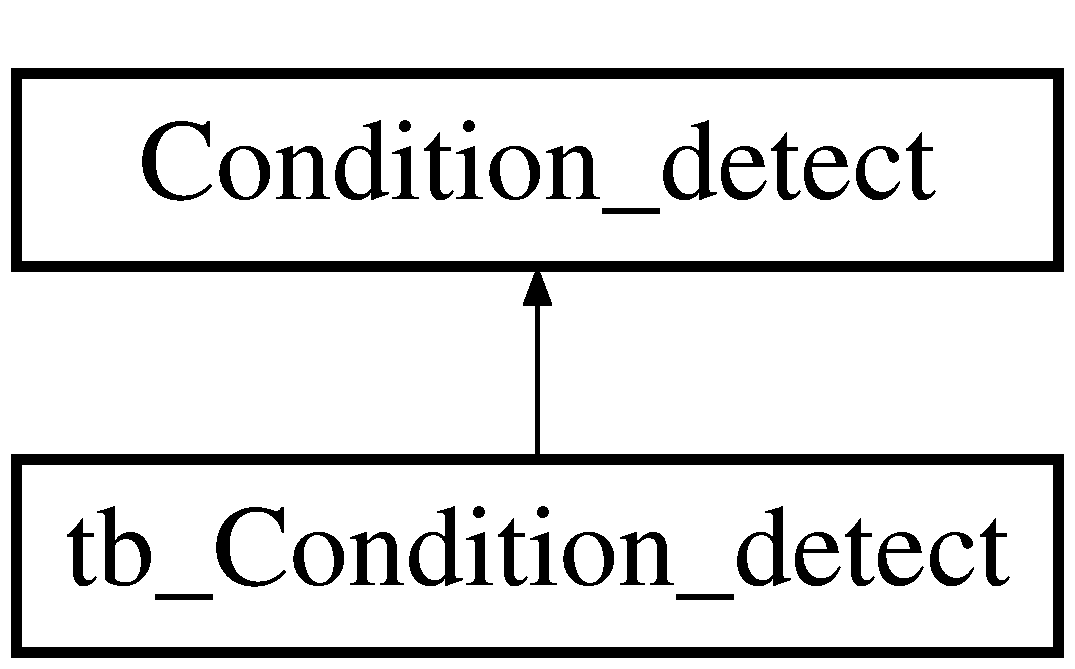
\includegraphics[height=2.000000cm]{class_condition__detect}
\end{center}
\end{figure}
\subsection*{Entities}
\begin{DoxyCompactItemize}
\item 
\hyperlink{class_condition__detect_1_1fsm}{fsm} architecture
\begin{DoxyCompactList}\small\item\em Architecture definition of the \hyperlink{class_condition__detect}{Condition\+\_\+detect}. \end{DoxyCompactList}\end{DoxyCompactItemize}
\subsection*{Libraries}
 \begin{DoxyCompactItemize}
\item 
\hyperlink{class_condition__detect_ae4f03c286607f3181e16b9aa12d0c6d4}{I\+E\+EE} 
\end{DoxyCompactItemize}
\subsection*{Use Clauses}
 \begin{DoxyCompactItemize}
\item 
\hyperlink{class_condition__detect_aa4b2b25246a821511120e3149b003563}{S\+T\+D\+\_\+\+L\+O\+G\+I\+C\+\_\+1164}   \hypertarget{class_condition__detect_aa4b2b25246a821511120e3149b003563}{}\label{class_condition__detect_aa4b2b25246a821511120e3149b003563}

\begin{DoxyCompactList}\small\item\em Use standard library. \end{DoxyCompactList}\end{DoxyCompactItemize}
\subsection*{Ports}
 \begin{DoxyCompactItemize}
\item 
\hyperlink{class_condition__detect_a6231b307b7958b6060563aa2a93d345a}{clk}  {\bfseries {\bfseries \textcolor{vhdlchar}{in}\textcolor{vhdlchar}{ }}} {\bfseries \textcolor{vhdlchar}{S\+T\+D\+\_\+\+L\+O\+G\+IC}\textcolor{vhdlchar}{ }} \hypertarget{class_condition__detect_a6231b307b7958b6060563aa2a93d345a}{}\label{class_condition__detect_a6231b307b7958b6060563aa2a93d345a}

\begin{DoxyCompactList}\small\item\em clock input \end{DoxyCompactList}\item 
\hyperlink{class_condition__detect_a3313e71ab116de6fc03014f85009a19d}{clk\+\_\+ena}  {\bfseries {\bfseries \textcolor{vhdlchar}{in}\textcolor{vhdlchar}{ }}} {\bfseries \textcolor{vhdlchar}{S\+T\+D\+\_\+\+L\+O\+G\+IC}\textcolor{vhdlchar}{ }} \hypertarget{class_condition__detect_a3313e71ab116de6fc03014f85009a19d}{}\label{class_condition__detect_a3313e71ab116de6fc03014f85009a19d}

\begin{DoxyCompactList}\small\item\em clock\+\_\+enable input \end{DoxyCompactList}\item 
\hyperlink{class_condition__detect_a3495b88db081463071853b171449fc35}{sync\+\_\+rst}  {\bfseries {\bfseries \textcolor{vhdlchar}{in}\textcolor{vhdlchar}{ }}} {\bfseries \textcolor{vhdlchar}{S\+T\+D\+\_\+\+L\+O\+G\+IC}\textcolor{vhdlchar}{ }} \hypertarget{class_condition__detect_a3495b88db081463071853b171449fc35}{}\label{class_condition__detect_a3495b88db081463071853b171449fc35}

\begin{DoxyCompactList}\small\item\em synchronization reset input \end{DoxyCompactList}\item 
\hyperlink{class_condition__detect_a8720760a9f71f283c56ace58995c6f62}{S\+C\+L\+\_\+in}  {\bfseries {\bfseries \textcolor{vhdlchar}{in}\textcolor{vhdlchar}{ }}} {\bfseries \textcolor{vhdlchar}{S\+T\+D\+\_\+\+L\+O\+G\+IC}\textcolor{vhdlchar}{ }} \hypertarget{class_condition__detect_a8720760a9f71f283c56ace58995c6f62}{}\label{class_condition__detect_a8720760a9f71f283c56ace58995c6f62}

\begin{DoxyCompactList}\small\item\em I2C clock line input. \end{DoxyCompactList}\item 
\hyperlink{class_condition__detect_a7779b5de6dcce1ecf9237a494bf3ed5f}{S\+D\+A\+\_\+in}  {\bfseries {\bfseries \textcolor{vhdlchar}{in}\textcolor{vhdlchar}{ }}} {\bfseries \textcolor{vhdlchar}{S\+T\+D\+\_\+\+L\+O\+G\+IC}\textcolor{vhdlchar}{ }} \hypertarget{class_condition__detect_a7779b5de6dcce1ecf9237a494bf3ed5f}{}\label{class_condition__detect_a7779b5de6dcce1ecf9237a494bf3ed5f}

\begin{DoxyCompactList}\small\item\em I2C data line input. \end{DoxyCompactList}\item 
\hyperlink{class_condition__detect_a6e8d259110b158dfc5a3b77d6bf5c838}{start\+\_\+detected\+\_\+point}  {\bfseries {\bfseries \textcolor{vhdlchar}{out}\textcolor{vhdlchar}{ }}} {\bfseries \textcolor{vhdlchar}{S\+T\+D\+\_\+\+L\+O\+G\+IC}\textcolor{vhdlchar}{ }} \hypertarget{class_condition__detect_a6e8d259110b158dfc5a3b77d6bf5c838}{}\label{class_condition__detect_a6e8d259110b158dfc5a3b77d6bf5c838}

\begin{DoxyCompactList}\small\item\em detected start condition \end{DoxyCompactList}\item 
\hyperlink{class_condition__detect_acefb7ff3520754727c54db5f8271c8ca}{stop\+\_\+detected\+\_\+point}  {\bfseries {\bfseries \textcolor{vhdlchar}{out}\textcolor{vhdlchar}{ }}} {\bfseries \textcolor{vhdlchar}{S\+T\+D\+\_\+\+L\+O\+G\+IC}\textcolor{vhdlchar}{ }} \hypertarget{class_condition__detect_acefb7ff3520754727c54db5f8271c8ca}{}\label{class_condition__detect_acefb7ff3520754727c54db5f8271c8ca}

\begin{DoxyCompactList}\small\item\em detected stop condition \end{DoxyCompactList}\item 
\hyperlink{class_condition__detect_a97379707029ffd9f27b8e1288ee2b963}{error\+\_\+detected\+\_\+point}  {\bfseries {\bfseries \textcolor{vhdlchar}{out}\textcolor{vhdlchar}{ }}} {\bfseries \textcolor{vhdlchar}{S\+T\+D\+\_\+\+L\+O\+G\+IC}\textcolor{vhdlchar}{ }} \hypertarget{class_condition__detect_a97379707029ffd9f27b8e1288ee2b963}{}\label{class_condition__detect_a97379707029ffd9f27b8e1288ee2b963}

\begin{DoxyCompactList}\small\item\em detected error condition \end{DoxyCompactList}\end{DoxyCompactItemize}


\subsection{Detailed Description}
Use logic elements \hyperlink{class_condition__detect}{Condition\+\_\+detect} entity brief description Detailed description of this \hyperlink{class_condition__detect}{Condition\+\_\+detect} design element. 

\subsection{Member Data Documentation}
\index{Condition\+\_\+detect@{Condition\+\_\+detect}!I\+E\+EE@{I\+E\+EE}}
\index{I\+E\+EE@{I\+E\+EE}!Condition\+\_\+detect@{Condition\+\_\+detect}}
\subsubsection[{\texorpdfstring{I\+E\+EE}{IEEE}}]{\setlength{\rightskip}{0pt plus 5cm}{\bf I\+E\+EE}\hspace{0.3cm}{\ttfamily [Library]}}\hypertarget{class_condition__detect_ae4f03c286607f3181e16b9aa12d0c6d4}{}\label{class_condition__detect_ae4f03c286607f3181e16b9aa12d0c6d4}
 

The documentation for this class was generated from the following file\+:\begin{DoxyCompactItemize}
\item 
C\+:/\+Users/\+Public/\+Documents/\+Github/\+V\+H\+D\+L/\+Condition\+\_\+detect/\hyperlink{_condition__detect_8vhd}{Condition\+\_\+detect.\+vhd}\end{DoxyCompactItemize}

\hypertarget{class_condition__detect_1_1fsm}{}\section{fsm Architecture Reference}
\label{class_condition__detect_1_1fsm}\index{fsm@{fsm}}


Architecture definition of the \hyperlink{class_condition__detect}{Condition\+\_\+detect}.  


\subsection*{Processes}
 \begin{DoxyCompactItemize}
\item 
\hyperlink{class_condition__detect_1_1fsm_aca869937c40a3cb0b3e8467b28f4c42b}{transitions\+\_\+and\+\_\+storage}{\bfseries  ( {\bfseries {\bfseries \hyperlink{class_condition__detect_a6231b307b7958b6060563aa2a93d345a}{clk}} \textcolor{vhdlchar}{ }} )}
\begin{DoxyCompactList}\small\item\em Process transitions\+\_\+and\+\_\+storage of the Architecture. \end{DoxyCompactList}\item 
\hyperlink{class_condition__detect_1_1fsm_ab52d69072c9e0a01dc1a2642b28297ab}{stateaction}{\bfseries  ( {\bfseries \textcolor{vhdlchar}{state}\textcolor{vhdlchar}{ }} )}\hypertarget{class_condition__detect_1_1fsm_ab52d69072c9e0a01dc1a2642b28297ab}{}\label{class_condition__detect_1_1fsm_ab52d69072c9e0a01dc1a2642b28297ab}

\begin{DoxyCompactList}\small\item\em if synchronization reset equals to 0 , state transfer to init state \end{DoxyCompactList}\end{DoxyCompactItemize}
\subsection*{Types}
 \begin{DoxyCompactItemize}
\item 
{\bfseries \hyperlink{class_condition__detect_1_1fsm_af1aa411452cee18437e460b9d30ed364}{t\+\_\+state}{\bfseries \textcolor{vhdlchar}{(}\textcolor{vhdlchar}{ }\textcolor{vhdlchar}{init}\textcolor{vhdlchar}{ }\textcolor{vhdlchar}{,}\textcolor{vhdlchar}{ }\textcolor{vhdlchar}{start\+\_\+detecting}\textcolor{vhdlchar}{ }\textcolor{vhdlchar}{,}\textcolor{vhdlchar}{ }\textcolor{vhdlchar}{start\+\_\+detected}\textcolor{vhdlchar}{ }\textcolor{vhdlchar}{,}\textcolor{vhdlchar}{ }\textcolor{vhdlchar}{stop\+\_\+detecting}\textcolor{vhdlchar}{ }\textcolor{vhdlchar}{,}\textcolor{vhdlchar}{ }\textcolor{vhdlchar}{stop\+\_\+detected}\textcolor{vhdlchar}{ }\textcolor{vhdlchar}{,}\textcolor{vhdlchar}{ }\textcolor{vhdlchar}{error}\textcolor{vhdlchar}{ }\textcolor{vhdlchar}{)}\textcolor{vhdlchar}{ }}} 
\end{DoxyCompactItemize}
\subsection*{Signals}
 \begin{DoxyCompactItemize}
\item 
\hyperlink{class_condition__detect_1_1fsm_a3faeb1655b4935d9040ff50adfdcd5f0}{state} {\bfseries {\bfseries \hyperlink{class_condition__detect_1_1fsm_af1aa411452cee18437e460b9d30ed364}{t\+\_\+state}} \textcolor{vhdlchar}{ }} \hypertarget{class_condition__detect_1_1fsm_a3faeb1655b4935d9040ff50adfdcd5f0}{}\label{class_condition__detect_1_1fsm_a3faeb1655b4935d9040ff50adfdcd5f0}

\end{DoxyCompactItemize}


\subsection{Detailed Description}
Architecture definition of the \hyperlink{class_condition__detect}{Condition\+\_\+detect}. 

More details about this \hyperlink{class_condition__detect}{Condition\+\_\+detect} element. 

\subsection{Member Function Documentation}
\index{Condition\+\_\+detect\+::fsm@{Condition\+\_\+detect\+::fsm}!transitions\+\_\+and\+\_\+storage@{transitions\+\_\+and\+\_\+storage}}
\index{transitions\+\_\+and\+\_\+storage@{transitions\+\_\+and\+\_\+storage}!Condition\+\_\+detect\+::fsm@{Condition\+\_\+detect\+::fsm}}
\subsubsection[{\texorpdfstring{transitions\+\_\+and\+\_\+storageclk}{transitions_and_storageclk}}]{\setlength{\rightskip}{0pt plus 5cm} {\bfseries \textcolor{vhdlchar}{ }} transitions\+\_\+and\+\_\+storage(
\begin{DoxyParamCaption}
\item[{}]{{\bfseries {\bfseries {\bf clk}} \textcolor{vhdlchar}{ }} {\em }}
\end{DoxyParamCaption}
)\hspace{0.3cm}{\ttfamily [Process]}}\hypertarget{class_condition__detect_1_1fsm_aca869937c40a3cb0b3e8467b28f4c42b}{}\label{class_condition__detect_1_1fsm_aca869937c40a3cb0b3e8467b28f4c42b}


Process transitions\+\_\+and\+\_\+storage of the Architecture. 

More details about this transitions\+\_\+and\+\_\+storage element. 

\subsection{Member Data Documentation}
\index{Condition\+\_\+detect\+::fsm@{Condition\+\_\+detect\+::fsm}!t\+\_\+state@{t\+\_\+state}}
\index{t\+\_\+state@{t\+\_\+state}!Condition\+\_\+detect\+::fsm@{Condition\+\_\+detect\+::fsm}}
\subsubsection[{\texorpdfstring{t\+\_\+state}{t_state}}]{\setlength{\rightskip}{0pt plus 5cm}{\bf t\+\_\+state} {\bfseries \textcolor{vhdlchar}{(}\textcolor{vhdlchar}{ }\textcolor{vhdlchar}{init}\textcolor{vhdlchar}{ }\textcolor{vhdlchar}{,}\textcolor{vhdlchar}{ }\textcolor{vhdlchar}{start\+\_\+detecting}\textcolor{vhdlchar}{ }\textcolor{vhdlchar}{,}\textcolor{vhdlchar}{ }\textcolor{vhdlchar}{start\+\_\+detected}\textcolor{vhdlchar}{ }\textcolor{vhdlchar}{,}\textcolor{vhdlchar}{ }\textcolor{vhdlchar}{stop\+\_\+detecting}\textcolor{vhdlchar}{ }\textcolor{vhdlchar}{,}\textcolor{vhdlchar}{ }\textcolor{vhdlchar}{stop\+\_\+detected}\textcolor{vhdlchar}{ }\textcolor{vhdlchar}{,}\textcolor{vhdlchar}{ }\textcolor{vhdlchar}{error}\textcolor{vhdlchar}{ }\textcolor{vhdlchar}{)}\textcolor{vhdlchar}{ }} \hspace{0.3cm}{\ttfamily [Type]}}\hypertarget{class_condition__detect_1_1fsm_af1aa411452cee18437e460b9d30ed364}{}\label{class_condition__detect_1_1fsm_af1aa411452cee18437e460b9d30ed364}
type t\+\_\+state as 6 differents states\+: init,start\+\_\+detecting,start\+\_\+detected,stop\+\_\+detecting,stop\+\_\+detected,error. 

The documentation for this class was generated from the following file\+:\begin{DoxyCompactItemize}
\item 
C\+:/\+Users/\+Public/\+Documents/\+Github/\+V\+H\+D\+L/\+Condition\+\_\+detect/\hyperlink{_condition__detect_8vhd}{Condition\+\_\+detect.\+vhd}\end{DoxyCompactItemize}

\hypertarget{classtb___condition__detect}{}\section{tb\+\_\+\+Condition\+\_\+detect Entity Reference}
\label{classtb___condition__detect}\index{tb\+\_\+\+Condition\+\_\+detect@{tb\+\_\+\+Condition\+\_\+detect}}
Inheritance diagram for tb\+\_\+\+Condition\+\_\+detect\+:\begin{figure}[H]
\begin{center}
\leavevmode
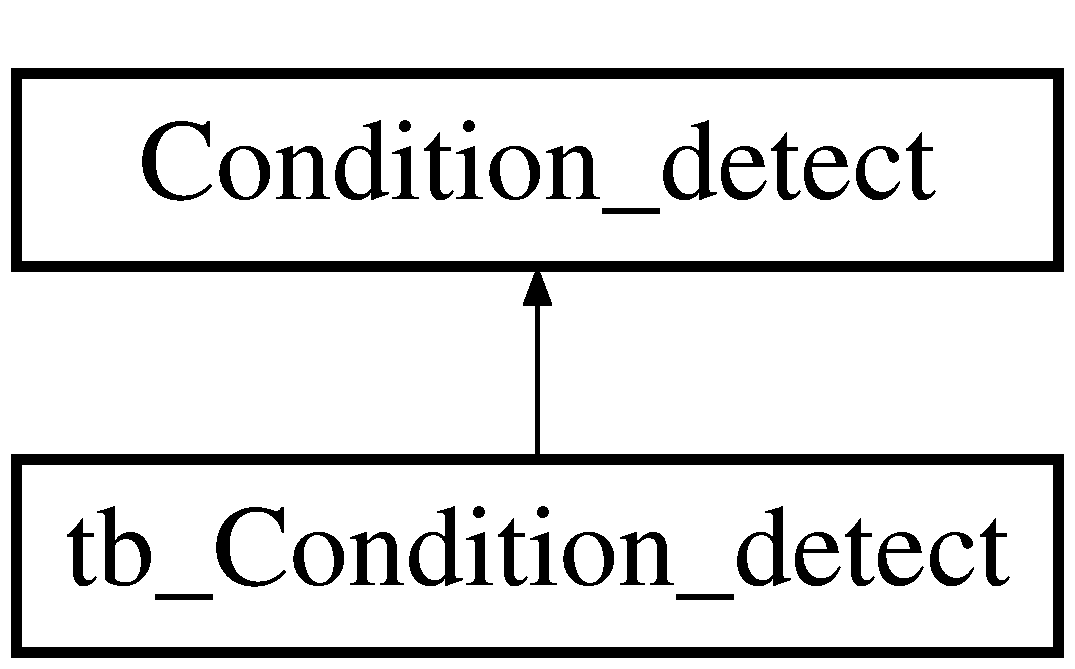
\includegraphics[height=2.000000cm]{classtb___condition__detect}
\end{center}
\end{figure}
\subsection*{Entities}
\begin{DoxyCompactItemize}
\item 
\hyperlink{classtb___condition__detect_1_1_behavioral}{Behavioral} architecture
\begin{DoxyCompactList}\small\item\em Architecture definition of the \hyperlink{classtb___condition__detect}{tb\+\_\+\+Condition\+\_\+detect}. \end{DoxyCompactList}\end{DoxyCompactItemize}
\subsection*{Libraries}
 \begin{DoxyCompactItemize}
\item 
\hyperlink{classtb___condition__detect_ae4f03c286607f3181e16b9aa12d0c6d4}{I\+E\+EE} \hypertarget{classtb___condition__detect_ae4f03c286607f3181e16b9aa12d0c6d4}{}\label{classtb___condition__detect_ae4f03c286607f3181e16b9aa12d0c6d4}

\begin{DoxyCompactList}\small\item\em Use standard library. \end{DoxyCompactList}\end{DoxyCompactItemize}
\subsection*{Use Clauses}
 \begin{DoxyCompactItemize}
\item 
\hyperlink{classtb___condition__detect_aa4b2b25246a821511120e3149b003563}{S\+T\+D\+\_\+\+L\+O\+G\+I\+C\+\_\+1164}   \hypertarget{classtb___condition__detect_aa4b2b25246a821511120e3149b003563}{}\label{classtb___condition__detect_aa4b2b25246a821511120e3149b003563}

\begin{DoxyCompactList}\small\item\em Use logic elements. \end{DoxyCompactList}\end{DoxyCompactItemize}


The documentation for this class was generated from the following file\+:\begin{DoxyCompactItemize}
\item 
C\+:/\+Users/\+Public/\+Documents/\+Github/\+V\+H\+D\+L/\+Condition\+\_\+detect/\hyperlink{tb___condition__detect_8vhd}{tb\+\_\+\+Condition\+\_\+detect.\+vhd}\end{DoxyCompactItemize}

\chapter{File Documentation}
\hypertarget{_condition__detect_8vhd}{}\section{C\+:/\+Users/\+Public/\+Documents/\+Github/\+V\+H\+D\+L/\+Condition\+\_\+detect/\+Condition\+\_\+detect.vhd File Reference}
\label{_condition__detect_8vhd}\index{C\+:/\+Users/\+Public/\+Documents/\+Github/\+V\+H\+D\+L/\+Condition\+\_\+detect/\+Condition\+\_\+detect.\+vhd@{C\+:/\+Users/\+Public/\+Documents/\+Github/\+V\+H\+D\+L/\+Condition\+\_\+detect/\+Condition\+\_\+detect.\+vhd}}


\hyperlink{class_condition__detect}{Condition\+\_\+detect} \+: This entity with synchronization reset is used to detect the condition of action from master by line S\+CL and S\+DA. According to the protocol of I2C, we need to use these two lines inputs. First, we need to judge the S\+DA data on every S\+CL high level. There are also three outputs to indicate these conditions. Stop condition means S\+DA from zero to one, start condition means S\+DA from one to zero. Start condition could be acted after the stop condition on the same S\+CL high level, that means restart condition. It\textquotesingle{}s same as a stop with a start. But, it can\textquotesingle{}t act the stop condition after the start condition , that makes no sense. And the state will transfer to init state. If it\textquotesingle{}s on S\+CL low level, it would also transfer to init state and waiting for the next judgement.  


\subsection*{Entities}
\begin{DoxyCompactItemize}
\item 
\hyperlink{class_condition__detect}{Condition\+\_\+detect} entity
\begin{DoxyCompactList}\small\item\em Use logic elements \hyperlink{class_condition__detect}{Condition\+\_\+detect} entity brief description Detailed description of this \hyperlink{class_condition__detect}{Condition\+\_\+detect} design element. \end{DoxyCompactList}\item 
\hyperlink{class_condition__detect_1_1fsm}{fsm} architecture
\begin{DoxyCompactList}\small\item\em Architecture definition of the \hyperlink{class_condition__detect}{Condition\+\_\+detect}. \end{DoxyCompactList}\end{DoxyCompactItemize}


\subsection{Detailed Description}
\hyperlink{class_condition__detect}{Condition\+\_\+detect} \+: This entity with synchronization reset is used to detect the condition of action from master by line S\+CL and S\+DA. According to the protocol of I2C, we need to use these two lines inputs. First, we need to judge the S\+DA data on every S\+CL high level. There are also three outputs to indicate these conditions. Stop condition means S\+DA from zero to one, start condition means S\+DA from one to zero. Start condition could be acted after the stop condition on the same S\+CL high level, that means restart condition. It\textquotesingle{}s same as a stop with a start. But, it can\textquotesingle{}t act the stop condition after the start condition , that makes no sense. And the state will transfer to init state. If it\textquotesingle{}s on S\+CL low level, it would also transfer to init state and waiting for the next judgement. 


\hypertarget{tb___condition__detect_8vhd}{}\section{C\+:/\+Users/\+Public/\+Documents/\+Github/\+V\+H\+D\+L/\+Condition\+\_\+detect/tb\+\_\+\+Condition\+\_\+detect.vhd File Reference}
\label{tb___condition__detect_8vhd}\index{C\+:/\+Users/\+Public/\+Documents/\+Github/\+V\+H\+D\+L/\+Condition\+\_\+detect/tb\+\_\+\+Condition\+\_\+detect.\+vhd@{C\+:/\+Users/\+Public/\+Documents/\+Github/\+V\+H\+D\+L/\+Condition\+\_\+detect/tb\+\_\+\+Condition\+\_\+detect.\+vhd}}


tb\+\_\+\+Condition\+\_\+detect\+\_\+\+Condition\+\_\+detect \+:testbench for the entity \hyperlink{class_condition__detect}{Condition\+\_\+detect}  


\subsection*{Entities}
\begin{DoxyCompactItemize}
\item 
\hyperlink{classtb___condition__detect}{tb\+\_\+\+Condition\+\_\+detect} entity
\item 
\hyperlink{classtb___condition__detect_1_1_behavioral}{Behavioral} architecture
\begin{DoxyCompactList}\small\item\em Architecture definition of the \hyperlink{classtb___condition__detect}{tb\+\_\+\+Condition\+\_\+detect}. \end{DoxyCompactList}\end{DoxyCompactItemize}


\subsection{Detailed Description}
tb\+\_\+\+Condition\+\_\+detect\+\_\+\+Condition\+\_\+detect \+:testbench for the entity \hyperlink{class_condition__detect}{Condition\+\_\+detect} 


%--- End generated contents ---

% Index
\backmatter
\newpage
\phantomsection
\clearemptydoublepage
\addcontentsline{toc}{chapter}{Index}
\printindex

\end{document}
